\documentclass[11pt]{article}


% --- Packages ---
\usepackage{amsmath, amsthm, amsfonts, amssymb, hyperref, soul, latexsym, stmaryrd, booktabs} % fonts and characters
\usepackage{enumitem, ytableau, comment, graphicx, makecell, appendix, titling, scrextend, float} % utilities
\usepackage{tikz, tikz-cd, tikzsymbols, pgfplots} % plots crap
\pgfplotsset{compat=1.18}
\usepackage{blkarray} % random math 
\usepackage{pstricks,pst-node,pst-tree} % networks
\usepackage{verbatim} % write code
\newlength\myverbindent % indent code
\setlength\myverbindent{0.5in} % change this to change indentation
\makeatletter
\def\verbatim@processline{%
  \hspace{\myverbindent}\the\verbatim@line\par}


% --- Formatting ---
\usepackage{fullpage} % margins
\usepackage{parskip} % whitespace between paragraphs, no indent

\numberwithin{equation}{section} % number equations with section number
\numberwithin{figure}{section} % number figure with section number
\numberwithin{table}{section} % number table with section number

\theoremstyle{definition}
\newtheorem{theorem}{Theorem}[section]
\newtheorem{lemma}[theorem]{Lemma}
\newtheorem{claim}[theorem]{Claim}
\newtheorem{conjecture}[theorem]{Conjecture}
\newtheorem{proposition}[theorem]{Proposition}
\newtheorem{corollary}[theorem]{Corollary}
\newtheorem{problem}[theorem]{Problem}
\newtheorem{exercise}[theorem]{Exercise}
\newtheorem{definition}[theorem]{Definition}

\newenvironment{solution}{\begin{addmargin}[2em]{0em} {\bf Solution. }}{\end{addmargin}}


% --- Math Crap ---
\newcommand{\E}{\mathbb{E}}
\newcommand{\Z}{\mathbb{Z}}
\newcommand{\R}{\mathbb{R}}
\newcommand{\Q}{\mathbb{Q}}
\newcommand{\C}{\mathbb{C}}
\newcommand{\N}{\mathbb{N}}
\newcommand{\lagr}{\mathcal{L}}
\newcommand{\e}{\varepsilon}
\renewcommand{\sup}{\text{sup}}
\renewcommand{\inf}{\text{inf}}
\renewcommand{\d}{\delta}
\renewcommand{\Re}{\text{Re}}
\renewcommand{\Im}{\text{Im}}
\newcommand{\Arg}{\text{Arg}}
\newcommand{\Log}{\text{Log}}
\newcommand{\conj}{\overline}
\newcommand{\intersection}{\cap}
\newcommand{\union}{\cup}


% --- Bibliography ---
%\usepackage[style=numeric, backend=biber]{biblatex} % packages
%\bibliography{filename} % .bib file


% --- Title ---
\title{Midterm}
\author{Gavin Engelstad et al.}
\date{\today}
\newcommand{\theclass}{Macro Modeling}
\newcommand{\theclassnum}{ECON 472}


% --- Document ---
\begin{document}
\noindent
{\theclass \hfill  \theauthor}\break
{\tiny \hspace*{\fill} \emph{Fix this}} \break
{\theclassnum  \hfill \thedate}

\begin{center}
	{\huge \textbf{\thetitle}}
\end{center}

\section{Habit Persistence}

Some economists argue that consumers like living the good life and they most often get used to it. Therefore, utility not only depends on current but also on \emph{previous} levels of consumption. Models like these are said to exhibit \emph{habit persistence in consumption} and have been fairly successful in accounting for several features of macro-finance data and in improving the fit of DSGE models.


\subsection{The Model Economy}

Consider an infinitely-lived economy consisting of a representative household and a representative firm. Assume that both the consumer and the firm are price takers. The household chooses infinite sequences of consumption $C_t$, investment $I_t$, and hours worked $N_t$ to maximize
\[
    \E \sum_{t=0}^\infty \beta^t u(C_t, C_{t-1}, N_t)
\]
where $\beta \in (0, 1)$ is the household's discount factor and where the instantaneous utility function $u$ takes the form
\[
    u(C_t, C_{t-1}, N_t) = \ln \left(C_t - \nu C_{t-1}\right) + \phi \left(1 - N_t\right).
\]

In the above, parameter $\nu \geq 0$ governs the household's habit persistence and parameter $\phi > 0$ governs the relative importance of consumption and leisure. The household's endowment consists of an initial capital stock $K_0$ and a (normalized) time endowment of 1 units of time every period, which it can devote either to work or leisure. Labor is paid at a rate $w_t$ per hour. Finally, assume that the household makes investment decisions each period, following the law of motion for capital
\[
    K_{t + 1} = (1 - \delta)K_t + I_t
\]
where $\delta \in [0, 1]$ is the depreciation rate of physical capital. Each period, the household rents capital $K_t$ to the representative firm and obtains a rental rate of $r_t$ per unit.

The representative firm uses a constant returns to scale technology $F$ to produce output, following:
\[
    Y_t = z_t F\left(K_{Ft}, N_{Ft}\right) = z_t K_{Ft}^\alpha N_{Ft}^{1-\alpha}.
\]

In the above, $z_t$ is a stochastic productivity shock, $K_{Ft}$ denotes the firm's capital input, and $N_{Ft}$ denotes its labor input. The process for $z_t$ follows
\[
    z_t =(1-\rho)z_{ss} + \rho z_{t-1} + \varepsilon_{zt},
\]
where $\rho \in (0,1)$, $z_{ss}$ is the steady-state level of the productivity shock, and $\varepsilon_{zt} \sim \mathcal{N}(0,\sigma_{z}^2)$.

\begin{exercise}
    What's the (economic) effect of habit persistence (alternatively, of parameter $\nu$)? In one or two paragraphs, provide an intuitive explanation and comment on whether you believe including a specification like this in a DSGE model makes sense. You don't have to do any analytical derivation, but be sure to thoroughly justify your answer. [10]
\end{exercise}

\begin{solution}
    I hate writing. I'll do this later.
\end{solution}


\begin{exercise}
    Set up the social planner problem associated to this economy. While you're at it, explain why you don't need to define a competitive equilibrium for this problem. [5]
\end{exercise}

\begin{solution}
    The solution to the Social Planner Problem is the set of household allocations $\{Y_t, K_{t+1}, C_t, I_t, N_t\}$ such that the households solve
    \begin{alignat*}{4}
        \text{max} \quad & U = \E_0 \sum_{t=0}^\infty \beta^t \left( \ln \left(C_t - \nu C_{t-1}\right) + \phi \left(1 - N_t\right) \right) \\
        \text{subject to} \quad & K_{t + 1} = (1 - \delta)K_t + I_t \\
        & C_t + I_t = Y_t \\
        & Y_t = z_t K_t^\alpha N_t^{1 - \alpha} \\
        & Y_t, K_{t+1}, C_t, I_t, N_t \geq 0.
    \end{alignat*}

    We can do this instead of a Competitive Equilibrium because the first and second welfare theorems hold since we have perfect competition and no distorting taxes.
\end{solution}


\begin{exercise}
    Use your answer to Exercise 1.2 to characterize the equilibrium of this economy. You'll see that the first-order condition for consumption is a bit more complicated than usual, so feel free to keep the Lagrange multiplier as an endogenous variable. [10]
\end{exercise}

\begin{solution}
    To make the first order conditions easier, we'll solve
    \begin{alignat*}{4}
        \text{max} \quad & U = \E_0 \sum_{t=0}^\infty \beta^t \left(\ln \left(C_t - \nu C_{t-1}\right) + \phi \left(1 - N_t\right)\right) \\
        \text{subject to} \quad & C_t + K_{t + 1} = z_t K_t^\alpha N_t^{1 - \alpha} + (1 - \delta)K_t \\
        & K_{t+1}, C_t, N_t \geq 0.
    \end{alignat*}

    This is easily shown to be equivalent to the earlier Social Planner Problem we set up earlier.

    Using this setup, the Lagrangian is
    \[
        \lagr = \E_0 \sum_{t=0}^\infty \beta^t \left( \ln \left(C_t - \nu C_{t-1}\right) + \phi \left(1 - N_t\right) + \lambda_t\left(z_t K_t^\alpha N_t^{1 - \alpha} + (1 - \delta)K_t - C_t - K_{t + 1}\right)\right).
    \]

    Solving this gets the set of first order conditions
    \begin{align*}
        \frac{\partial \lagr}{\partial K_{t+1}} &= \beta^{t+1} \lambda_{t+1} \left(z_{t+1} \alpha K_{t+1}^{\alpha-1} N_{t+1}^{1-\alpha} + (1 - \delta)\right) - \beta^t \lambda_t \\
        \frac{\partial \lagr}{\partial C_t} &= \beta^t \left(\frac{1}{C_t - \nu C_{t-1}} - \lambda_t\right) - \beta^{t+1} \frac{\nu}{C_{t+1} - \nu C_t} \\
        \frac{\partial \lagr}{\partial N_t} &= \beta^t \left((1-\alpha) \lambda_t z_t K_t^\alpha N_t^{-\alpha}-\phi \right) \\
        \frac{\partial \lagr}{\partial \lambda_t} &= \beta^t \left(z_t K_t^\alpha N_t^{1 - \alpha} + (1 - \delta)K_t - C_t - K_{t + 1}\right).
    \end{align*}

    To simplify this again, we add the conditions
    \begin{align*}
        Y_t &= z_t K_t^\alpha N_t^{1-\alpha} \\
        r_t &= \alpha z_t K_t^{\alpha - 1} N_t^{1 - \alpha} \\
        w_t &= (1 - \alpha) z_t K_t^\alpha N_t^{-\alpha} \\
        I_t &= K_{t + 1} - (1 - \delta) K_t,
    \end{align*}
    rearrange, and set the FOCs to zero to get the system
    \begin{align*}
        Y_t &= z_t K_t^\alpha N_t^{1-\alpha} \\
        r_t &= \alpha Y_t K_t^{-1} \\
        w_t &= (1 - \alpha) Y_t N_t^{-1} \\
        I_t &= K_{t + 1} - (1 - \delta) K_t \\
        Y_t &= C_t + I_t \\
        \lambda_t &= \frac{1}{C_t - \nu C_{t-1}} - \frac{\beta \nu}{C_{t+1} - \nu C_t} \\
        \phi &= \lambda_t w_t \\
        \lambda_t &= \beta (\lambda_{t+1} r_{t+1} + (1-\delta) \lambda_{t+1}).
    \end{align*} 
\end{solution}


\begin{exercise}
    Use your answer to Exercise 1.3 to find the closed-form solutions to the steady state values for all the economy's variables. You should set $z_{ss} = 1$. [10]
\end{exercise}

\begin{solution}
    Setting everything in the system equal to their steady state values gets the system
    \begin{align*}
        Y_{ss} &= z_{ss} K_{ss}^\alpha N_{ss}^{1-\alpha} \\
        r_{ss} &= \alpha Y_{ss} K_{ss}^{-1} \\
        w_{ss} &= (1 - \alpha) Y_{ss} N_{ss}^{-1} \\
        I_{ss} &= K_{ss} - (1 - \delta) K_{ss} \\
        Y_{ss} &= C_{ss} + I_{ss} \\
        \lambda_{ss} &= \frac{1}{C_{ss} - \nu C_{ss}} - \frac{\beta \nu}{C_{ss} - \nu C_{ss}} \\
        \phi &= \lambda_{ss} w_{ss} \\
        \lambda_{ss} &= \beta(\lambda_{ss} r_{ss} + (1-\delta) \lambda_{ss}).
    \end{align*}

    Doing some hellish algebra\footnote{Check out Appendix \ref{sec:ss}.} to solve these gets
    \begin{align*}
        r_{ss} &= \frac{1}{\beta} - 1 + \delta \\
        K_{ss} &= z_{ss}^{\frac{1}{1-\alpha}}\frac{(1-\alpha)(1-\beta \nu)}{\phi (1 - \nu) \left(\frac{r_{ss}}{\alpha} - \delta\right)} \left(\frac{r_{ss}}{\alpha}\right)^{\frac{\alpha}{\alpha-1}} \\
        Y_{ss} &= \frac{r_{ss}}{\alpha} K_{ss} \\
        C_{ss} &= \left(\frac{r_{ss}}{\alpha} - \delta\right) K_{ss}\\
        I_{ss} &= \delta K_{ss} \\
        N_{ss} &= \left(\frac{r_{ss}}{\alpha z_{ss}}\right)^{\frac{1}{1-\alpha}} K_{ss} \\
        w_{ss} &= \frac{\phi (1-\nu)}{1-\beta\nu} \left(\frac{r_{ss}}{\alpha} - \delta\right) K_{ss}\\
        \lambda_{ss} &= \frac{1 - \beta\nu}{(1-\nu) C_{ss}}
    \end{align*}
\end{solution}


\begin{exercise}
    Use your answer to Exercise 1.3 and Uhlig's rules to log-linearize the equations that characterize the equilibrium of this economy.
\end{exercise}

\begin{solution}
    The equations become\footnote{For derivations see Appendix \ref{sec:ll}}
    \begin{align*}
        Y_t &= z_t K_t^\alpha N_t^{1-\alpha} &\implies&& \hat{Y}_t &= \hat{z}_t + \alpha \hat{K}_t + (1-\alpha) \hat{N}_t \\
        r_t &= \alpha Y_t K_t^{-1} &\implies&& \hat{r}_t &= \hat{Y}_t - \hat{K}_t \\
        w_t &= (1 - \alpha) Y_t N_t^{-1} &\implies&& \hat{w}_t &= \hat{Y}_t - \hat{N}_t \\
        I_t &= K_{t + 1} - (1 - \delta) K_t &\implies&& I_{ss} \hat{I}_t &= K_{ss} \hat{K}_{t + 1} - (1 - \delta) K_{ss} \hat{K}_t \\
        Y_t &= C_t + I_t &\implies&& Y_{ss} \hat{Y}_t &= C_{ss} \hat{C}_t + I_{ss} \hat{I}_t \\
        \lambda_t &= \frac{1}{C_t - \nu C_{t-1}} - \frac{\beta \nu}{C_{t+1} - \nu C_t} &\implies&& \lambda_{ss} \hat{\lambda}_t &= \frac{\nu}{(1 - \nu)^2 C_{ss}} \hat{C}_{t-1} + \frac{\beta \nu}{(1 - \nu)^2 C_{ss}} \hat{C}_{t+1} - \frac{1 + \beta \nu^2}{(1 - \nu)^2 C_{ss}} \hat{C}_t \\
        \phi &= \lambda_t w_t &\implies&& 0 &= \hat{\lambda}_t + \hat{w}_t \\
        \lambda_t &= \beta(\lambda_{t+1} r_{t+1} + (1-\delta) \lambda_{t+1}) &\implies&& \lambda_{ss} \hat{\lambda}_t &= \beta \lambda_{ss} (r_{ss} + 1 - \delta) \hat{\lambda}_{t+1} + \beta \lambda_{ss} r_{ss} \hat{r}_{t+1}.
    \end{align*} 

    We also have the law of motion for TFP, which becomes
    \begin{align*}
        z_t &= (1-\rho)z_{ss} + \rho z_{t-1} + \varepsilon_{zt} &\implies&& \hat{z}_t &= \rho \hat{z}_{t-1} + \varepsilon_{zt}
    \end{align*}
\end{solution}


\begin{exercise}
    Use your answer to Exercise 1.5 to map the log-linearized equilibrium conditions into the system of matrix equations
    \begin{align*}
        \vec{0} &= \mathbf{A} \vec{x}_{t+1} + \mathbf{B} \vec{x}_t + \mathbf{C} \vec{y}_t + \mathbf{D} \vec{z}_t \\
        \vec 0 &= \mathbb{E} \left[ \mathbf{F} \vec{x}_{t+2} + \mathbf{G} \vec{x}_{t+1} + \mathbf{H} \vec{x}_t + \mathbf{J} \vec{y}_{t+1} + \mathbf{K} \vec{y}_t + \mathbf{L} \vec{z}_{t+1} + \mathbf{M} \vec{z}_t \right] \\
        \vec{z}_{t+1} &= \mathbf{N} \vec{z}_t + \vec{e}_{t+1}
    \end{align*}
    where $\vec{x}_t$ is an $(m \times 1)$ vector of endogenous state variables, $z_t$ is a $(k \times 1)$ vector of exogenous state variables, and $y_t$ is an $(n \times 1)$ vector of other endogenous variables. [15]
\end{exercise}

\begin{solution}
    Let
    \[
        \vec{x}_t = \begin{pmatrix}
            \hat{K}_t \\
            \hat{C}_t
        \end{pmatrix}, \vec{y}_t = \begin{pmatrix}
            \hat{Y}_t \\
            \hat{I}_t \\
            \hat{N}_t \\
            \hat{r}_t \\
            \hat{w}_t \\
            \hat{\lambda}_t
        \end{pmatrix}, \vec{z}_t = \begin{pmatrix}
            \hat{z}_t
        \end{pmatrix}.
    \]

    The matrices are
    \begin{align*}
        &\mathbf{A} = \begin{pmatrix}
            0 & 0 \\
            0 & 0 \\
            0 & 0 \\
            K_{ss} & 0 \\
            0 & 0 \\
            0 & 0
        \end{pmatrix}, \mathbf{B} = \begin{pmatrix}
            \alpha & 0 \\
            -1 & 0 \\
            0 & 0 \\
            -(1-\delta) K_{ss} & 0 \\
            0 & C_{ss} \\
            0 & 0
        \end{pmatrix}, \mathbf{C} = \begin{pmatrix}
            -1 & 0 & (1-\alpha) & 0 & 0 & 0 \\
            1 & 0 & 0 & -1 & 0 & 0 \\
            1 & 0 & -1 & 0 & -1 & 0 \\
            0 & -I_{ss} & 0 & 0 & 0 & 0 \\
            -Y_{ss} & I_{ss} & 0 & 0 & 0 & 0 \\
            0 & 0 & 0 & 0 & 1 & 1
        \end{pmatrix}, \\
        &\mathbf{D} = \begin{pmatrix}
            1 \\ 0 \\ 0 \\ 0 \\ 0 \\ 0
       \end{pmatrix}
    \end{align*}
    in the first equation,
    \begin{align*}
        &\mathbf{F} = \begin{pmatrix}
            0 & \frac{\beta \nu}{(1 - \nu)^2 C_{ss}} \\
            0 & 0
        \end{pmatrix}, \mathbf{G} = \begin{pmatrix}
            0 & -\frac{1 + \beta \nu^2}{(1 - \nu)^2 C_{ss}} \\
            0 & 0
        \end{pmatrix}, \mathbf{H} = \begin{pmatrix}
            0 & \frac{\nu}{(1 - \nu)^2 C_{ss}} \\
            0 & 0
        \end{pmatrix} \\
        &\mathbf{J} = \begin{pmatrix}
            0 & 0 & 0 & 0 & 0 & -\lambda_{ss} \\
            0 & 0 & 0 & \beta \lambda_{ss} r_{ss} & 0 & \beta \lambda_{ss} (r_{ss} + 1 - \delta)
        \end{pmatrix}, \mathbf{K} = \begin{pmatrix}
            0 & 0 & 0 & 0 & 0 & 0 \\
            0 & 0 & 0 & 0 & 0 & -\lambda_{ss}
        \end{pmatrix}, \mathbf{L} = \begin{pmatrix}
            0 \\ 0
        \end{pmatrix}, \\
        &\mathbf{M} = \begin{pmatrix}
            0 \\ 0
        \end{pmatrix}
    \end{align*}
    in the second equation, and
    \[
        \mathbf{N} = \begin{pmatrix}
            \rho
        \end{pmatrix}, \vec{e}_{t+1} = \begin{pmatrix}
            \varepsilon_{zt}
        \end{pmatrix}
    \]
    in the last one.\footnote{Check out Appendix \ref{sec:mat} for the setup.}


\end{solution}


\begin{exercise}
    Let $\beta=0.9$, $\nu=0.85$, $\phi=0.5$, $\delta=0.1$, $\alpha=0.36$,and $\rho=0.95$. Use the \verb+uc_xyz+ function from the \verb+macro_modeling+ module and your answer to Exercise 1.6 to derive the matrices $\{\mathbf{P}, \mathbf{Q}, \mathbf{R}, \mathbf{S}\}$ that yield the policy functions
    \begin{align*}
        \vec{x}_{t+1} &= \mathbf{P} \vec{x}_t + \mathbf{Q} \vec{z}_t \\
        \vec{y}_t &= \mathbf{R} \vec{x}_t + \mathbf{S} \vec{z}_t 
    \end{align*}
    Offer a brief interpretation of your findings. If you think it is useful, you may write out the policy functions for each variable in $x_t$ and $y_t$. [15]
\end{exercise}

\begin{solution}
    I got the system
    \begin{align*}
        \begin{pmatrix}
            \hat{K}_{t+1} \\
            \hat{C}_{t+1}
        \end{pmatrix} &= \begin{pmatrix}
            0.77940762 & 0.05395422\\
            0.04173628 & 0.81810069\\
          \end{pmatrix} \begin{pmatrix}
            \hat{K}_t \\
            \hat{C}_t
        \end{pmatrix} + \begin{pmatrix}
            0.32412304\\
            0.18995039\\
          \end{pmatrix} \begin{pmatrix}
            \hat{z}_t
        \end{pmatrix} \\
        \begin{pmatrix}
            \hat{Y}_t \\
            \hat{I}_t \\
            \hat{N}_t \\
            \hat{r}_t \\
            \hat{w}_t \\
            \hat{\lambda}_t
        \end{pmatrix} &= \begin{pmatrix}
            -0.20564175 & 0.92147982\\
            -1.20592382 & 0.53954217\\
            -0.88381523 & 1.43981222\\
            -1.20564175 & 0.92147982\\
            0.67817348 & -0.5183324\\
            -0.67817348 & 0.5183324\\
          \end{pmatrix} \begin{pmatrix}
            \hat{K}_t \\
            \hat{C}_t
        \end{pmatrix} + \begin{pmatrix}
            0.55271507\\
            3.24123037\\
            -0.6988827\\
            0.55271507\\
            1.25159777\\
            -1.25159777\\
          \end{pmatrix} \begin{pmatrix}
            \hat{z}_t
        \end{pmatrix}.
    \end{align*}

    This suggests that $\hat{K}_{t+1}$ and $\hat{C}_{t+1}$ are increasing with respect to $\hat{K}_t$ and $\hat{C}_t$ (since the coefficients are positive), but do regress closer to the steady state (since they are less than 1). They also are increasing with $\hat{z}_t$, suggesting that they'll behave procyclically.

    Similarly, we find that $\hat{Y}_t$, $\hat{I}_t$, $\hat{r}_t$, and $\hat{w}_t$ behave procyclically, since the $\hat{z}_t$ coefficient is positive. $\hat{N}_t$ (and $\hat{\lambda}_t$) behave countercyclical, suggesting that when labor output (and output in general) is more efficient, households take advantage by having more leisure.
\end{solution}


\begin{exercise}
    Use your answer to Exercise 1.7 to plot the impulse-response functions of output, consumption, hours worked, and investment in response to a TFP shock. Are TFP shocks still consistent with the business cycle facts? \emph{Hint}: strictly speaking, you don't need Python to answer this question. [10]
\end{exercise}

\begin{solution}
    I got the below figure.

    \begin{figure}[H]
        \centering
        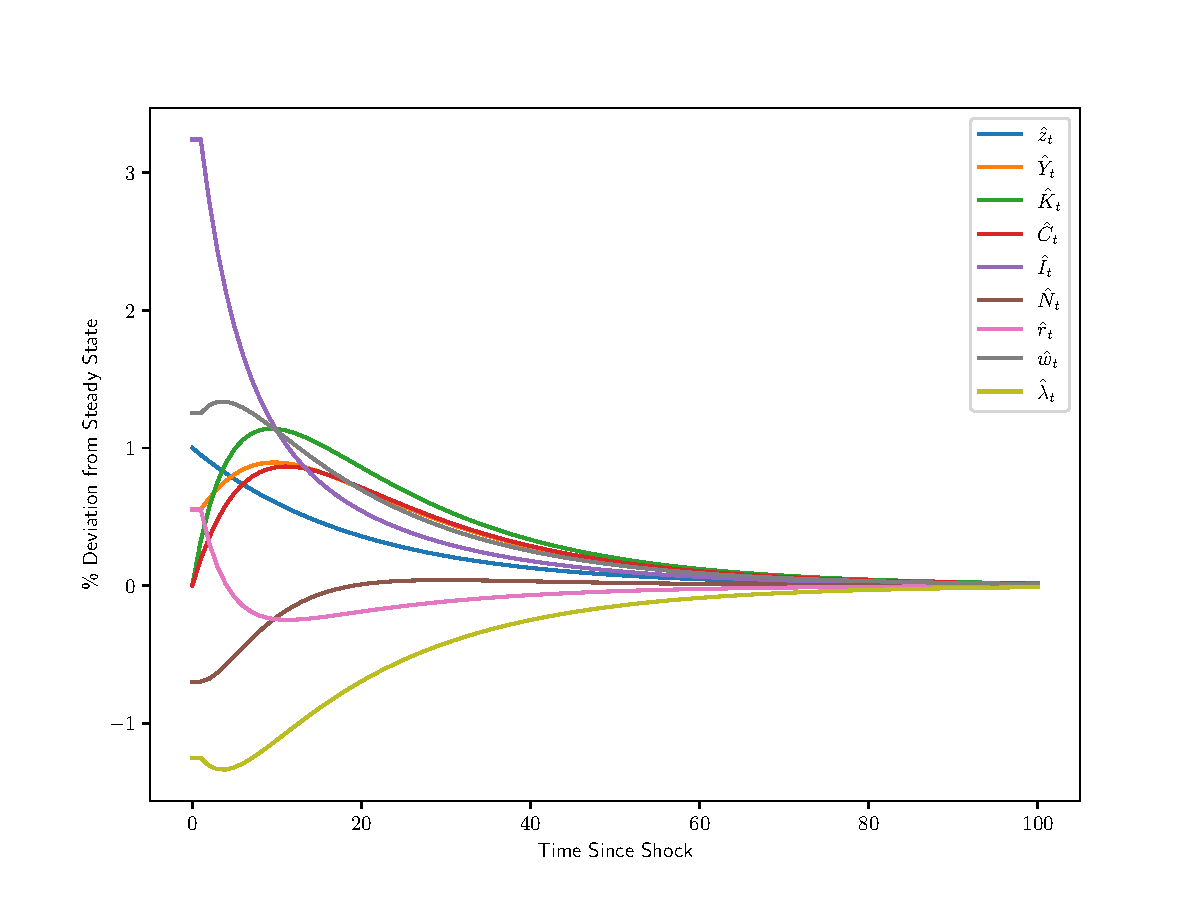
\includegraphics[width=\textwidth]{graphs/nu=0.85.pdf}
    \end{figure}
\end{solution}


\begin{exercise}
    Redo Exercise 1.8 under the assumption that $\nu = 0$ (this is, there is no habit persistence, which is the baseline we've covered in class so far). Compare the impulse-response functions of both specifications. How are they different? This is an open-ended question, but a good answer should look at how the impulse-response functions differ in amplitude (i.e., how large are the changes plotted in your graph) and persistence (i.e., for how many periods are the changes different from zero). [5]
\end{exercise}

\begin{solution}
    TBD
\end{solution}


\clearpage
\appendix
\appendixpage

\section{Steady State Derivation}\label{sec:ss}

This was awful and not fun.

Start with 
\begin{align}
    Y_{ss} &= z_{ss} K_{ss}^\alpha N_{ss}^{1-\alpha} \label{eq:ss1} \\
    r_{ss} &= \alpha Y_{ss} K_{ss}^{-1} \label{eq:ss2} \\
    w_{ss} &= (1 - \alpha) Y_{ss} N_{ss}^{-1} \label{eq:ss3} \\
    I_{ss} &= K_{ss} - (1 - \delta) K_{ss} \label{eq:ss4} \\
    Y_{ss} &= C_{ss} + I_{ss} \label{eq:ss5} \\
    \lambda_{ss} &= \frac{1}{C_{ss} - \nu C_{ss}} - \frac{\beta \nu}{C_{ss} - \nu C_{ss}} \label{eq:ss6} \\
    \phi &= \lambda_{ss} w_{ss} \label{eq:ss7} \\
    \lambda_{ss} &= \beta(\lambda_{ss} r_{ss} + (1-\delta) \lambda_{ss}). \label{eq:ss8}
\end{align}

$\lambda_{ss}$ cancels in \ref{eq:ss8} to get
\[
    1 = \beta (r_{ss} + 1 - \delta)
\]
which means
\[
    r_{ss} = \frac{1}{\beta} - 1 + \delta.
\]

\ref{eq:ss6} becomes
\[
    \lambda_{ss} = \frac{1}{C_{ss} - \nu C_{ss}} - \frac{\beta \nu}{C_{ss} - \nu C_{ss}} = \frac{1 - \beta \nu}{(1-\nu) C_{ss}}.
\]

For the next equations, we use the ``solve everything for $K$ and hope for the best'' strategy.

Starting with \ref{eq:ss4}, that gets
\[
    I_{ss} = K_{ss} - (1 - \delta) K_{ss} = \delta K_{ss}.
\]

Then, treating $r_{ss}$ as solved, \ref{eq:ss2} is
\[
    r_{ss} = \alpha Y_{ss} K_{ss}^{-1},
\]
which becomes
\[
    Y_{ss} = \frac{r_{ss}}{\alpha} K_{ss}.
\]

Plugging the expression for $Y_{ss}$ and $z_{ss} = 1$ into \ref{eq:ss1} gets
\[
    \frac{r_{ss}}{\alpha} K_{ss} = z_{ss} K_{ss}^\alpha N_{ss}^{1-\alpha}.
\]
Dividing this by $K_{ss}^\alpha$ gets
\[
    \frac{r_{ss}}{\alpha z_{ss}} K_{ss}^{1-\alpha} = N_{ss}^{1-\alpha},
\]
which when raised to the $\frac{1}{1-\alpha}$ power gets
\[
    N_{ss} = \left(\frac{r_{ss}}{\alpha z_{ss}}\right)^{\frac{1}{1-\alpha}} K_{ss}.
\]

Using the expressions for $Y_{ss}$ and $I_{ss}$ in \ref{eq:ss5} gets
\[
    \frac{r_{ss}}{\alpha} K_{ss} = C_{ss} + \delta K_ss,
\]
which simplifies to
\[
    C_{ss} = \left(\frac{r_{ss}}{\alpha} - \delta\right) K_{ss}.
\]

Finally, plugging the expression for $\lambda_{ss}$ into \ref{eq:ss7} gets
\[
    \phi = \frac{1 - \beta \nu}{(1-\nu) C_{ss}} w_{ss},
\]
which becomes
\[
    w_{ss} = \frac{\phi (1-\nu)}{1-\beta\nu} C_{ss} = \frac{\phi (1-\nu)}{1-\beta\nu} \left(\frac{r_{ss}}{\alpha} - \delta\right) K_{ss}.
\]

Finally, plugging everything into \ref{eq:ss3} gets
\[
    \frac{\phi (1-\nu)}{1-\beta\nu} \left(\frac{r_{ss}}{\alpha} - \delta\right) K_{ss} = (1-\alpha) \left(\frac{r_{ss}}{\alpha} K_{ss}\right)\left(\left(\frac{r_{ss}}{\alpha z_{ss}}\right)^{\frac{1}{1-\alpha}} K_{ss}\right)^{-1} = (1-\alpha) z_{ss}^{\frac{1}{1-\alpha}} \left(\frac{r_{ss}}{\alpha}\right)^{\frac{\alpha}{\alpha-1}},
\]
which gets the solution
\[
    K_{ss} = z_{ss}^{\frac{1}{1-\alpha}} \frac{(1-\alpha)(1-\beta \nu)}{\phi (1 - \nu) \left(\frac{r_{ss}}{\alpha} - \delta\right)} \left(\frac{r_{ss}}{\alpha}\right)^{\frac{\alpha}{\alpha-1}}.
\]

Using the expression for $r_{ss}$, we can find $K_{ss}$ and can plug in values backwards to get all the other variables.


\section{Log-Linearizing Everything} \label{sec:ll}

Mario, I've done more algebra for this than any of my math classes.

Start with the system
\begin{align}
    Y_t &= z_t K_t^\alpha N_t^{1-\alpha} \label{eq:ll1} \\
    r_t &= \alpha Y_t K_t^{-1} \label{eq:ll2} \\
    w_t &= (1 - \alpha) Y_t N_t^{-1} \label{eq:ll3} \\
    I_t &= K_{t + 1} - (1 - \delta) K_t \label{eq:ll4} \\
    Y_t &= C_t + I_t \label{eq:ll5} \\
    \lambda_t &= \frac{1}{C_t - \nu C_{t-1}} - \frac{\beta \nu}{C_{t+1} - \nu C_t} \label{eq:ll6} \\
    \phi &= \lambda_t w_t \label{eq:ll7} \\
    \lambda_t &= \beta(\lambda_{t+1} r_{t+1} + (1-\delta) \lambda_{t+1}). \label{eq:ll8}
\end{align}

Moving top to bottom, \ref{eq:ll1} becomes
\[
    Y_{ss} (1+\hat{Y}_t) = z_{ss} K_{ss}^\alpha N_{ss}^{1-\alpha} (1 + \hat{z}_t + \alpha \hat{K}_t + (1-\alpha) \hat{N}_t).
\]
Canceling \ref{eq:ss1} and subtracting 1 from both sides gets
\[
    \hat{Y}_t = \hat{z}_t + \alpha \hat{K}_t + (1-\alpha) \hat{N}_t.
\]

\ref{eq:ll2} becomes
\[
    r_{ss} (1 + \hat{r}_t) = \alpha Y_{ss} K_{ss}^{-1} (1 + \hat{Y}_t - \hat{K}_t).
\]
Canceling \ref{eq:ss2} and subtracting 1 from both sides gets\footnote{This is going to get really repetitive.}
\[
    \hat{r}_t = \hat{Y}_t - \hat{K}_t.
\]

\ref{eq:ll3} becomes
\[
    w_{ss} (1 + \hat{w}_t) = (1 - \alpha) Y_{ss} N_{ss}^{-1} (1 + \hat{Y}_t - \hat{N}_t),
\]
which when we cancel \ref{eq:ss3} and subtract 1 gets
\[
    \hat{w}_t = \hat{Y}_t - \hat{N}_t.
\]

\ref{eq:ll4} becomes
\[
    I_{ss} (1 + \hat{I}_t) = K_{ss} (1 + \hat{K}_{t + 1}) - (1 - \delta) K_{ss} (1 + \hat{K}_t),
\]
which means
\[
    I_{ss} + I_{ss} \hat{I}_t = K_{ss} + K_{ss} \hat{K}_{t + 1} - (1 - \delta) K_{ss} - (1 - \delta) K_{ss} \hat{K}_t.
\]
Canceling \ref{eq:ss4} gets
\[
    I_{ss} \hat{I}_t = K_{ss} \hat{K}_{t + 1} - (1 - \delta) K_{ss} \hat{K}_t.
\]

\ref{eq:ll5} becomes
\[
    Y_ss (1 + \hat{Y}_t) = C_{ss} (1 + \hat{C}_t) + I_{ss} (1 + \hat{I}_t),
\]
which when expanded is
\[
    Y_ss + Y_{ss} \hat{Y}_t = C_{ss} + C_{ss} \hat{C}_t + I_{ss} + I_{ss} \hat{I}_t.
\]
Canceling \ref{eq:ss5} gets
\[
    Y_{ss} \hat{Y}_t = C_{ss} \hat{C}_t + I_{ss} \hat{I}_t.
\]

Before we log-linearize \ref{eq:ll6}, we define
\[
    X_t = C_t - \nu C_{t-1}
\]
so that\footnote{
    Want proof? We create
    \[
        X_{ss} (1 + \hat{X}_t) = C_{ss} (1 + \hat{C}_t) - \nu C_{ss} (1 + \hat{C}_{t-1}),
    \]
    which cancels with the steady state equation
    \[
        X_{ss} = C_{ss} - \nu C_{ss}.
    \]
    to get
    \[
        X_{ss} \hat{X}_t = C_{ss} \hat{C}_t - \nu C_{ss} \hat{C}_{t-1}.
    \]
}
\[
    X_{ss} \hat{X}_t = C_{ss} \hat{C}_t - \nu C_{ss} \hat{C}_{t-1}
\]

Plugging $X_t$ into \ref{eq:ll6} gets
\[
    \lambda_t = \frac{1}{X_{t}} - \frac{\beta \nu}{X_{t+1}} = X_{t}^{-1} - \beta \nu X_{t+1}^{-1}.
\]
This becomes
\[
    \lambda_{ss} (1 + \hat{\lambda}_t) = X_{ss}^{-1} (1 - \hat{X}_t) - \beta \nu X_{ss}^{-1} (1 - \hat{X}_{t+1}).
\]
Canceling the steady state equation
\[
    \lambda_{ss} = X_{ss}^{-1} - \beta \nu X_{ss}^{-1}
\]
gets
\[
    \lambda_{ss} \hat{\lambda}_t = \beta \nu X_{ss}^{-1} \hat{X}_{t+1} - X_{ss}^{-1} \hat{X}_t.
\]
Plugging in 
\[
    X_{ss}^{-1} \hat{X}_t = \frac{1}{(1 - \nu)^2 C_{ss}} \hat{C}_t - \frac{\nu}{(1 - \nu)^2 C_{ss}} \hat{C}_{t-1}
\]
gets the final log-linearized system
\begin{align*}
    \lambda_{ss} \hat{\lambda}_t &= \frac{\beta \nu}{(1 - \nu)^2 C_{ss}} \hat{C}_{t+1} - \frac{\beta \nu^2}{(1 - \nu)^2 C_{ss}} \hat{C}_t - \frac{1}{(1 - \nu)^2 C_{ss}} \hat{C}_t + \frac{\nu}{(1 - \nu)^2 C_{ss}} \hat{C}_{t-1} \\
    &= \frac{\nu}{(1 - \nu)^2 C_{ss}} \hat{C}_{t-1} + \frac{\beta \nu}{(1 - \nu)^2 C_{ss}} \hat{C}_{t+1} - \frac{1 + \beta \nu^2}{(1 - \nu)^2 C_{ss}} \hat{C}_t.
\end{align*}

\ref{eq:ll7} becomes
\[
    \phi = \lambda_{ss} w_{ss} (1 + \hat{\lambda}_t + \hat{w}_t),
\]
which canceling \ref{eq:ss7} and subtracting 1 becomes
\[
    0 = \hat{\lambda}_t + \hat{w}_t.
\]

Finally, \ref{eq:ll8} becomes
\[
    \lambda_{ss} (1 + \hat{\lambda}_t) = \beta \lambda_{ss} r_{ss} (1 + \hat{\lambda}_{t+1} + \hat{r}_{t+1}) + \beta (1-\delta) \lambda_{ss} (1 + \hat{\lambda}_{t+1}),
\]
which means
\[
    \lambda_{ss} + \lambda_{ss} \hat{\lambda}_t = \beta \lambda_{ss} r_{ss} + \beta \lambda_{ss} r_{ss} \hat{\lambda}_{t+1} + \beta \lambda_{ss} r_{ss} \hat{r}_{t+1} + \beta (1-\delta) \lambda_{ss} + \beta (1-\delta) \lambda_{ss} \hat{\lambda}_{t+1}.
\]
Canceling \ref{eq:ss8} from this gets
\[
    \lambda_{ss} \hat{\lambda}_t = \beta \lambda_{ss} (r_{ss} + 1 - \delta) \hat{\lambda}_{t+1} + \beta \lambda_{ss} r_{ss} \hat{r}_{t+1}.
\]

To log-linearize the law of motion for TFP, we start with
\[
    z_t = (1-\rho) z_{ss} + \rho z_{t-1} + \varepsilon_{zt}.
\]
Then, we turn it into
\[
    z_{ss}(1 + \hat{z}_t) = (1-\rho) z_{ss} + \rho z_{ss} (1 + \hat{z}_{t-1}) + \varepsilon_{zt}.
\]
Subtracting $z_{ss}$ on both sides gets
\[
    \hat{z}_t = \rho \hat{z}_{t-1} + \varepsilon_{zt}
\]


\section{Creating the Matrices} \label{sec:mat}

The first matrix equation,
\[
    \vec{0} = \mathbf{A} \vec{x}_{t+1} + \mathbf{B} \vec{x}_t + \mathbf{C} \vec{y}_t + \mathbf{D} \vec{z}_t,
\]
will include the equations
\begin{align*}
    \hat{Y}_t &= \hat{z}_t + \alpha \hat{K}_t + (1-\alpha) \hat{N}_t \\
    \hat{r}_t &= \hat{Y}_t - \hat{K}_t \\
    \hat{w}_t &= \hat{Y}_t - \hat{N}_t \\
    I_{ss} \hat{I}_t &= K_{ss} \hat{K}_{t + 1} - (1 - \delta) K_{ss} \hat{K}_t \\
    Y_{ss} \hat{Y}_t &= C_{ss} \hat{C}_t + I_{ss} \hat{I}_t \\
    0 &= \hat{\lambda}_t + \hat{w}_t
\end{align*}
Therefore, it becomes
\begin{align*}
    \begin{pmatrix}
        0 \\ 0 \\ 0 \\ 0 \\ 0 \\ 0
    \end{pmatrix} = &\begin{pmatrix}
        0 & 0 \\
        0 & 0 \\
        0 & 0 \\
        K_{ss} & 0 \\
        0 & 0 \\
        0 & 0
    \end{pmatrix} \begin{pmatrix}
        \hat{K}_{t+1} \\
        \hat{C}_{t+1}
    \end{pmatrix} + \begin{pmatrix}
        \alpha & 0 \\
        -1 & 0 \\
        0 & 0 \\
        -(1-\delta) K_{ss} & 0 \\
        0 & C_{ss} \\
        0 & 0
    \end{pmatrix} \begin{pmatrix}
        \hat{K}_t \\
        \hat{C}_t
    \end{pmatrix} \\
    &+ \begin{pmatrix}
        -1 & 0 & (1-\alpha) & 0 & 0 & 0 \\
        1 & 0 & 0 & -1 & 0 & 0 \\
        1 & 0 & -1 & 0 & -1 & 0 \\
        0 & -I_{ss} & 0 & 0 & 0 & 0 \\
        -Y_{ss} & I_{ss} & 0 & 0 & 0 & 0 \\
        0 & 0 & 0 & 0 & 1 & 1
    \end{pmatrix} \begin{pmatrix}
        \hat{Y}_t \\
        \hat{I}_t \\
        \hat{N}_t \\
        \hat{r}_t \\
        \hat{w}_t \\
        \hat{\lambda}_t
    \end{pmatrix} + \begin{pmatrix}
         1 \\ 0 \\ 0 \\ 0 \\ 0 \\ 0
    \end{pmatrix} \begin{pmatrix}
        \hat{z}_t
    \end{pmatrix}.
\end{align*}
Thus,
\begin{align*}
    &\mathbf{A} = \begin{pmatrix}
        0 & 0 \\
        0 & 0 \\
        0 & 0 \\
        K_{ss} & 0 \\
        0 & 0 \\
        0 & 0
    \end{pmatrix}, \mathbf{B} = \begin{pmatrix}
        \alpha & 0 \\
        -1 & 0 \\
        0 & 0 \\
        -(1-\delta) K_{ss} & 0 \\
        0 & C_{ss} \\
        0 & 0
    \end{pmatrix}, \mathbf{C} = \begin{pmatrix}
        -1 & 0 & (1-\alpha) & 0 & 0 & 0 \\
        1 & 0 & 0 & -1 & 0 & 0 \\
        1 & 0 & -1 & 0 & -1 & 0 \\
        0 & -I_{ss} & 0 & 0 & 0 & 0 \\
        -Y_{ss} & I_{ss} & 0 & 0 & 0 & 0 \\
        0 & 0 & 0 & 0 & 1 & 1
    \end{pmatrix}, \\
    &\mathbf{D} = \begin{pmatrix}
        1 \\ 0 \\ 0 \\ 0 \\ 0 \\ 0
   \end{pmatrix}.
\end{align*}

The second matrix equation,
\[
    \vec 0 = \mathbb{E} \left[ \mathbf{F} \vec{x}_{t+2} + \mathbf{G} \vec{x}_{t+1} + \mathbf{H} \vec{x}_t + \mathbf{J} \vec{y}_{t+1} + \mathbf{K} \vec{y}_t + \mathbf{L} \vec{z}_{t+1} + \mathbf{M} \vec{z}_t \right],
\]
will include the equations\footnote{The time is shifted one period forward from the log-linearized version in the first one.}
\begin{align*}
    \lambda_{ss} \hat{\lambda}_{t+1} &= \frac{\nu}{(1 - \nu)^2 C_{ss}} \hat{C}_t + \frac{\beta \nu}{(1 - \nu)^2 C_{ss}} \hat{C}_{t+2} - \frac{1 + \beta \nu^2}{(1 - \nu)^2 C_{ss}} \hat{C}_{t+1} \\
    \lambda_{ss} \hat{\lambda}_t &= \beta \lambda_{ss} (r_{ss} + 1 - \delta) \hat{\lambda}_{t+1} + \beta \lambda_{ss} r_{ss} \hat{r}_{t+1}.
\end{align*}
Therefore, it becomes
\begin{align*}
    \begin{pmatrix}
        0 \\ 0
    \end{pmatrix} = &\E \left[ \begin{pmatrix}
        0 & \frac{\beta \nu}{(1 - \nu)^2 C_{ss}} \\
        0 & 0
    \end{pmatrix} \begin{pmatrix}
        \hat{K}_{t+2} \\
        \hat{C}_{t+2}
    \end{pmatrix} + \begin{pmatrix}
        0 & -\frac{1 + \beta \nu^2}{(1 - \nu)^2 C_{ss}} \\
        0 & 0
    \end{pmatrix} \begin{pmatrix}
        \hat{K}_{t+1} \\
        \hat{C}_{t+1}
    \end{pmatrix} + \begin{pmatrix}
        0 & \frac{\nu}{(1 - \nu)^2 C_{ss}} \\
        0 & 0
    \end{pmatrix} \begin{pmatrix}
        \hat{K}_t \\
        \hat{C}_t
    \end{pmatrix}
    \right. \\
    &+ \begin{pmatrix}
        0 & 0 & 0 & 0 & 0 & -\lambda_{ss} \\
        0 & 0 & 0 & \beta \lambda_{ss} r_{ss} & 0 & \beta \lambda_{ss} (r_{ss} + 1 - \delta)
    \end{pmatrix} \begin{pmatrix}
        \hat{Y}_{t+1} \\
        \hat{I}_{t+1} \\
        \hat{N}_{t+1} \\
        \hat{r}_{t+1} \\
        \hat{w}_{t+1} \\
        \hat{\lambda}_{t+1}
    \end{pmatrix} + \begin{pmatrix}
        0 & 0 & 0 & 0 & 0 & 0 \\
        0 & 0 & 0 & 0 & 0 & -\lambda_{ss}
    \end{pmatrix} \begin{pmatrix}
        \hat{Y}_t \\
        \hat{I}_t \\
        \hat{N}_t \\
        \hat{r}_t \\
        \hat{w}_t \\
        \hat{\lambda}_t
    \end{pmatrix} \\
    &+ \left.\begin{pmatrix}
        0 \\ 0
    \end{pmatrix} \begin{pmatrix}
        \hat{z}_{t+1}
    \end{pmatrix} + \begin{pmatrix}
        0 \\ 0
    \end{pmatrix} \begin{pmatrix}
        \hat{z}_t
    \end{pmatrix} \right]
\end{align*}
Thus,
\begin{align*}
    &\mathbf{F} = \begin{pmatrix}
        0 & \frac{\beta \nu}{(1 - \nu)^2 C_{ss}} \\
        0 & 0
    \end{pmatrix}, \mathbf{G} = \begin{pmatrix}
        0 & -\frac{1 + \beta \nu^2}{(1 - \nu)^2 C_{ss}} \\
        0 & 0
    \end{pmatrix}, \mathbf{H} = \begin{pmatrix}
        0 & \frac{\nu}{(1 - \nu)^2 C_{ss}} \\
        0 & 0
    \end{pmatrix} \\
    &\mathbf{J} = \begin{pmatrix}
        0 & 0 & 0 & 0 & 0 & -\lambda_{ss} \\
        0 & 0 & 0 & \beta \lambda_{ss} r_{ss} & 0 & \beta \lambda_{ss} (r_{ss} + 1 - \delta)
    \end{pmatrix}, \mathbf{K} = \begin{pmatrix}
        0 & 0 & 0 & 0 & 0 & 0 \\
        0 & 0 & 0 & 0 & 0 & -\lambda_{ss}
    \end{pmatrix}, \mathbf{L} = \begin{pmatrix}
        0 \\ 0
    \end{pmatrix}, \\
    &\mathbf{M} = \begin{pmatrix}
        0 \\ 0
    \end{pmatrix}
\end{align*}

Finally, the last matrix equation,
\[
    \vec{z}_{t+1} = \mathbf{N} \vec{z}_t + \vec{e}_{t+1}
\]
will include the law of motion for TFP,
\[
    \hat{z}_t = \rho \hat{z}_{t-1} + \varepsilon_{zt}.
\]
Therefore, it becomes
\[
    \begin{pmatrix}
        \hat{z}_{t+1}
    \end{pmatrix} = \begin{pmatrix}
        \rho
    \end{pmatrix} \begin{pmatrix}
        \hat{z}_t
    \end{pmatrix} + \begin{pmatrix}
        \varepsilon_{zt}
    \end{pmatrix}.
\]
Thus,
\[
    \mathbf{N} = \begin{pmatrix}
        \rho
    \end{pmatrix}, \vec{e}_{t+1} = \begin{pmatrix}
        \varepsilon_{zt}
    \end{pmatrix}.
\]

\end{document}